\section{Sequence Diagram}\label{sec:sequenze}

I diagrammi di sequenza descrivono tre flussi significativi di DriveHub e mostrano come presentazione, servizi, dominio e persistenza collaborano nel tempo. Le chiamate ai servizi partono dai controller JavaFX e attraversano \code{ServiceUiGateway}: nel diagramma dell'acquisizione il gateway ha una linea di vita, mentre negli altri due è indicato in una nota. La linea «UnitOfWork / DAO» raccoglie l'apertura della transazione tramite \code{DaoFactory}, le chiamate ai DAO sulla stessa connessione e il commit. I diagrammi sono stati disegnati selezionando le operazioni effettive nei metodi di servizio, non generati automaticamente dai sorgenti.

\subsection{Acquisto di un veicolo}

\begin{figure}[H]
  \centering
  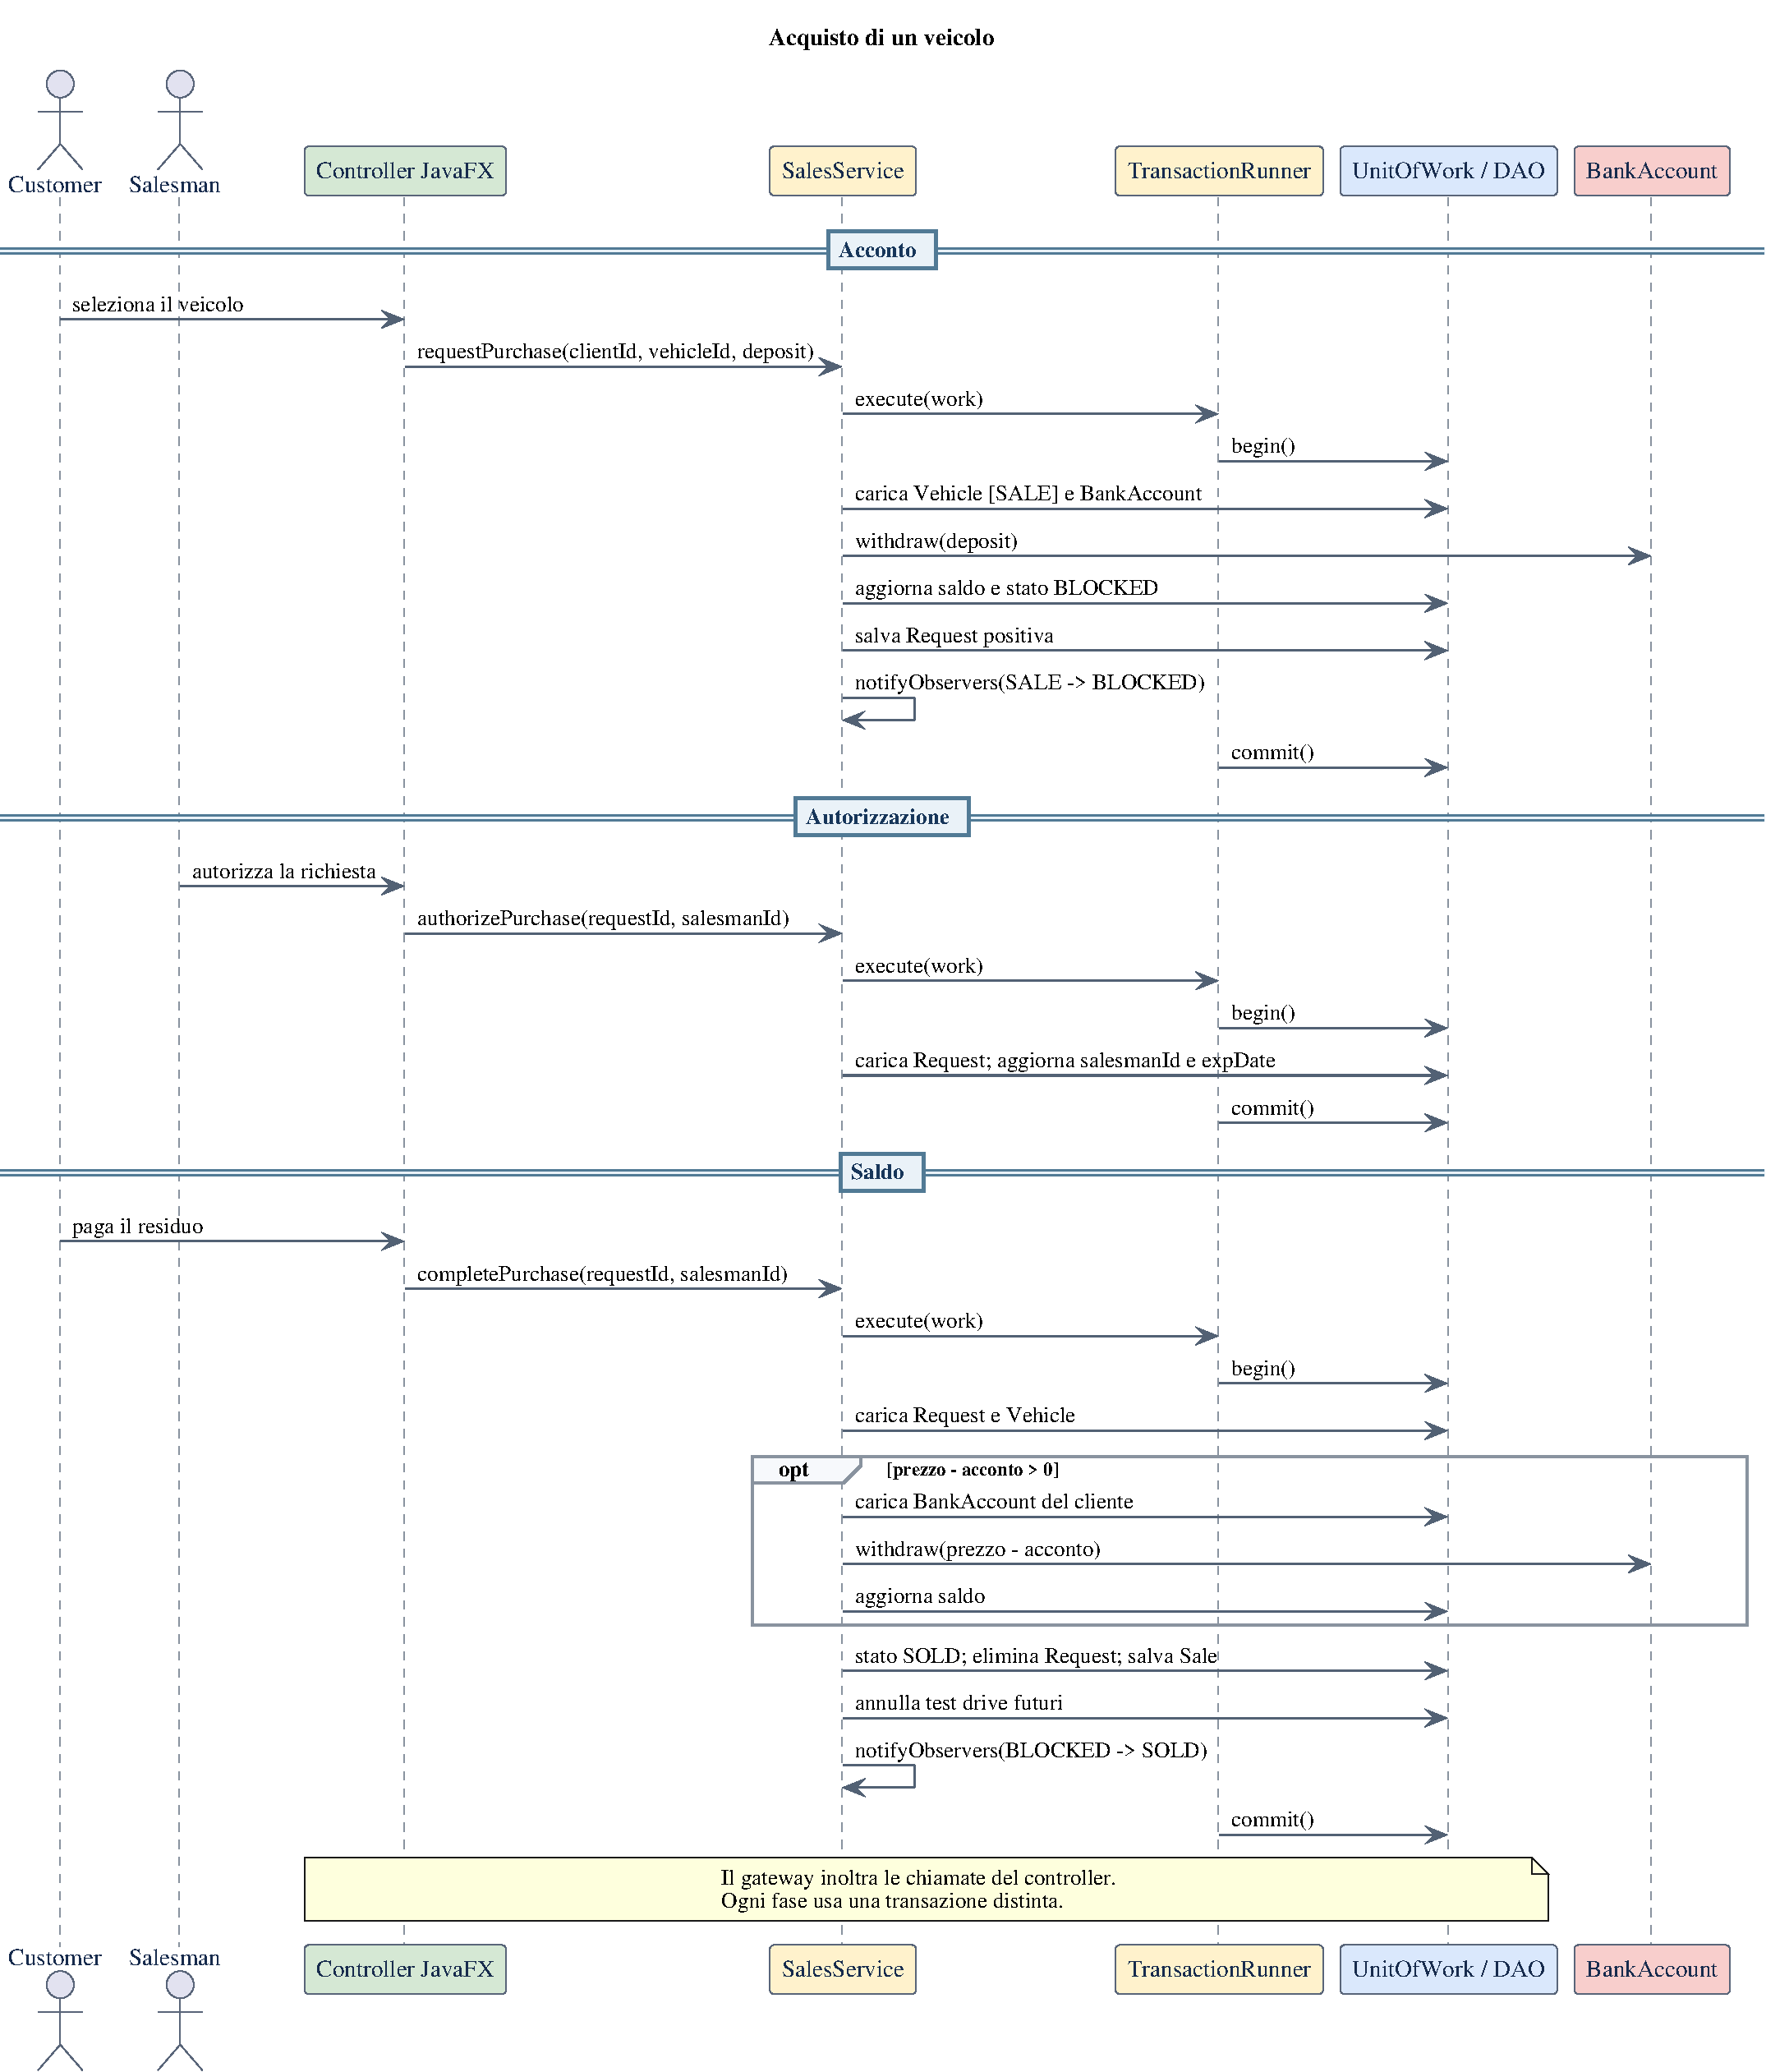
\includegraphics[width=\textwidth,height=.72\textheight,keepaspectratio]{sequence-purchase-drivehub.pdf}
  \caption{Acquisto: acconto del Customer, autorizzazione del Salesman e saldo finale.}\label{fig:seq-purchase}
\end{figure}

La figura~\ref{fig:seq-purchase} distingue tre transazioni. La prima verifica lo stato \code{SALE}, addebita l'acconto sul conto dimostrativo, porta il veicolo a \code{BLOCKED} e salva una \code{Request} positiva. Il Salesman imposta poi il proprio ID e una scadenza di un mese. Infine \code{SalesService} addebita al cliente della richiesta il residuo (prezzo meno acconto), registra la \code{Sale}, elimina la \code{Request} e annulla i test drive futuri prima del commit. Il controller abilita il saldo dopo l'autorizzazione, ma \code{completePurchase} non ricontrolla scadenza né identità del chiamante.

\clearpage
\subsection{Prenotazione di un noleggio}

\begin{figure}[H]
  \centering
  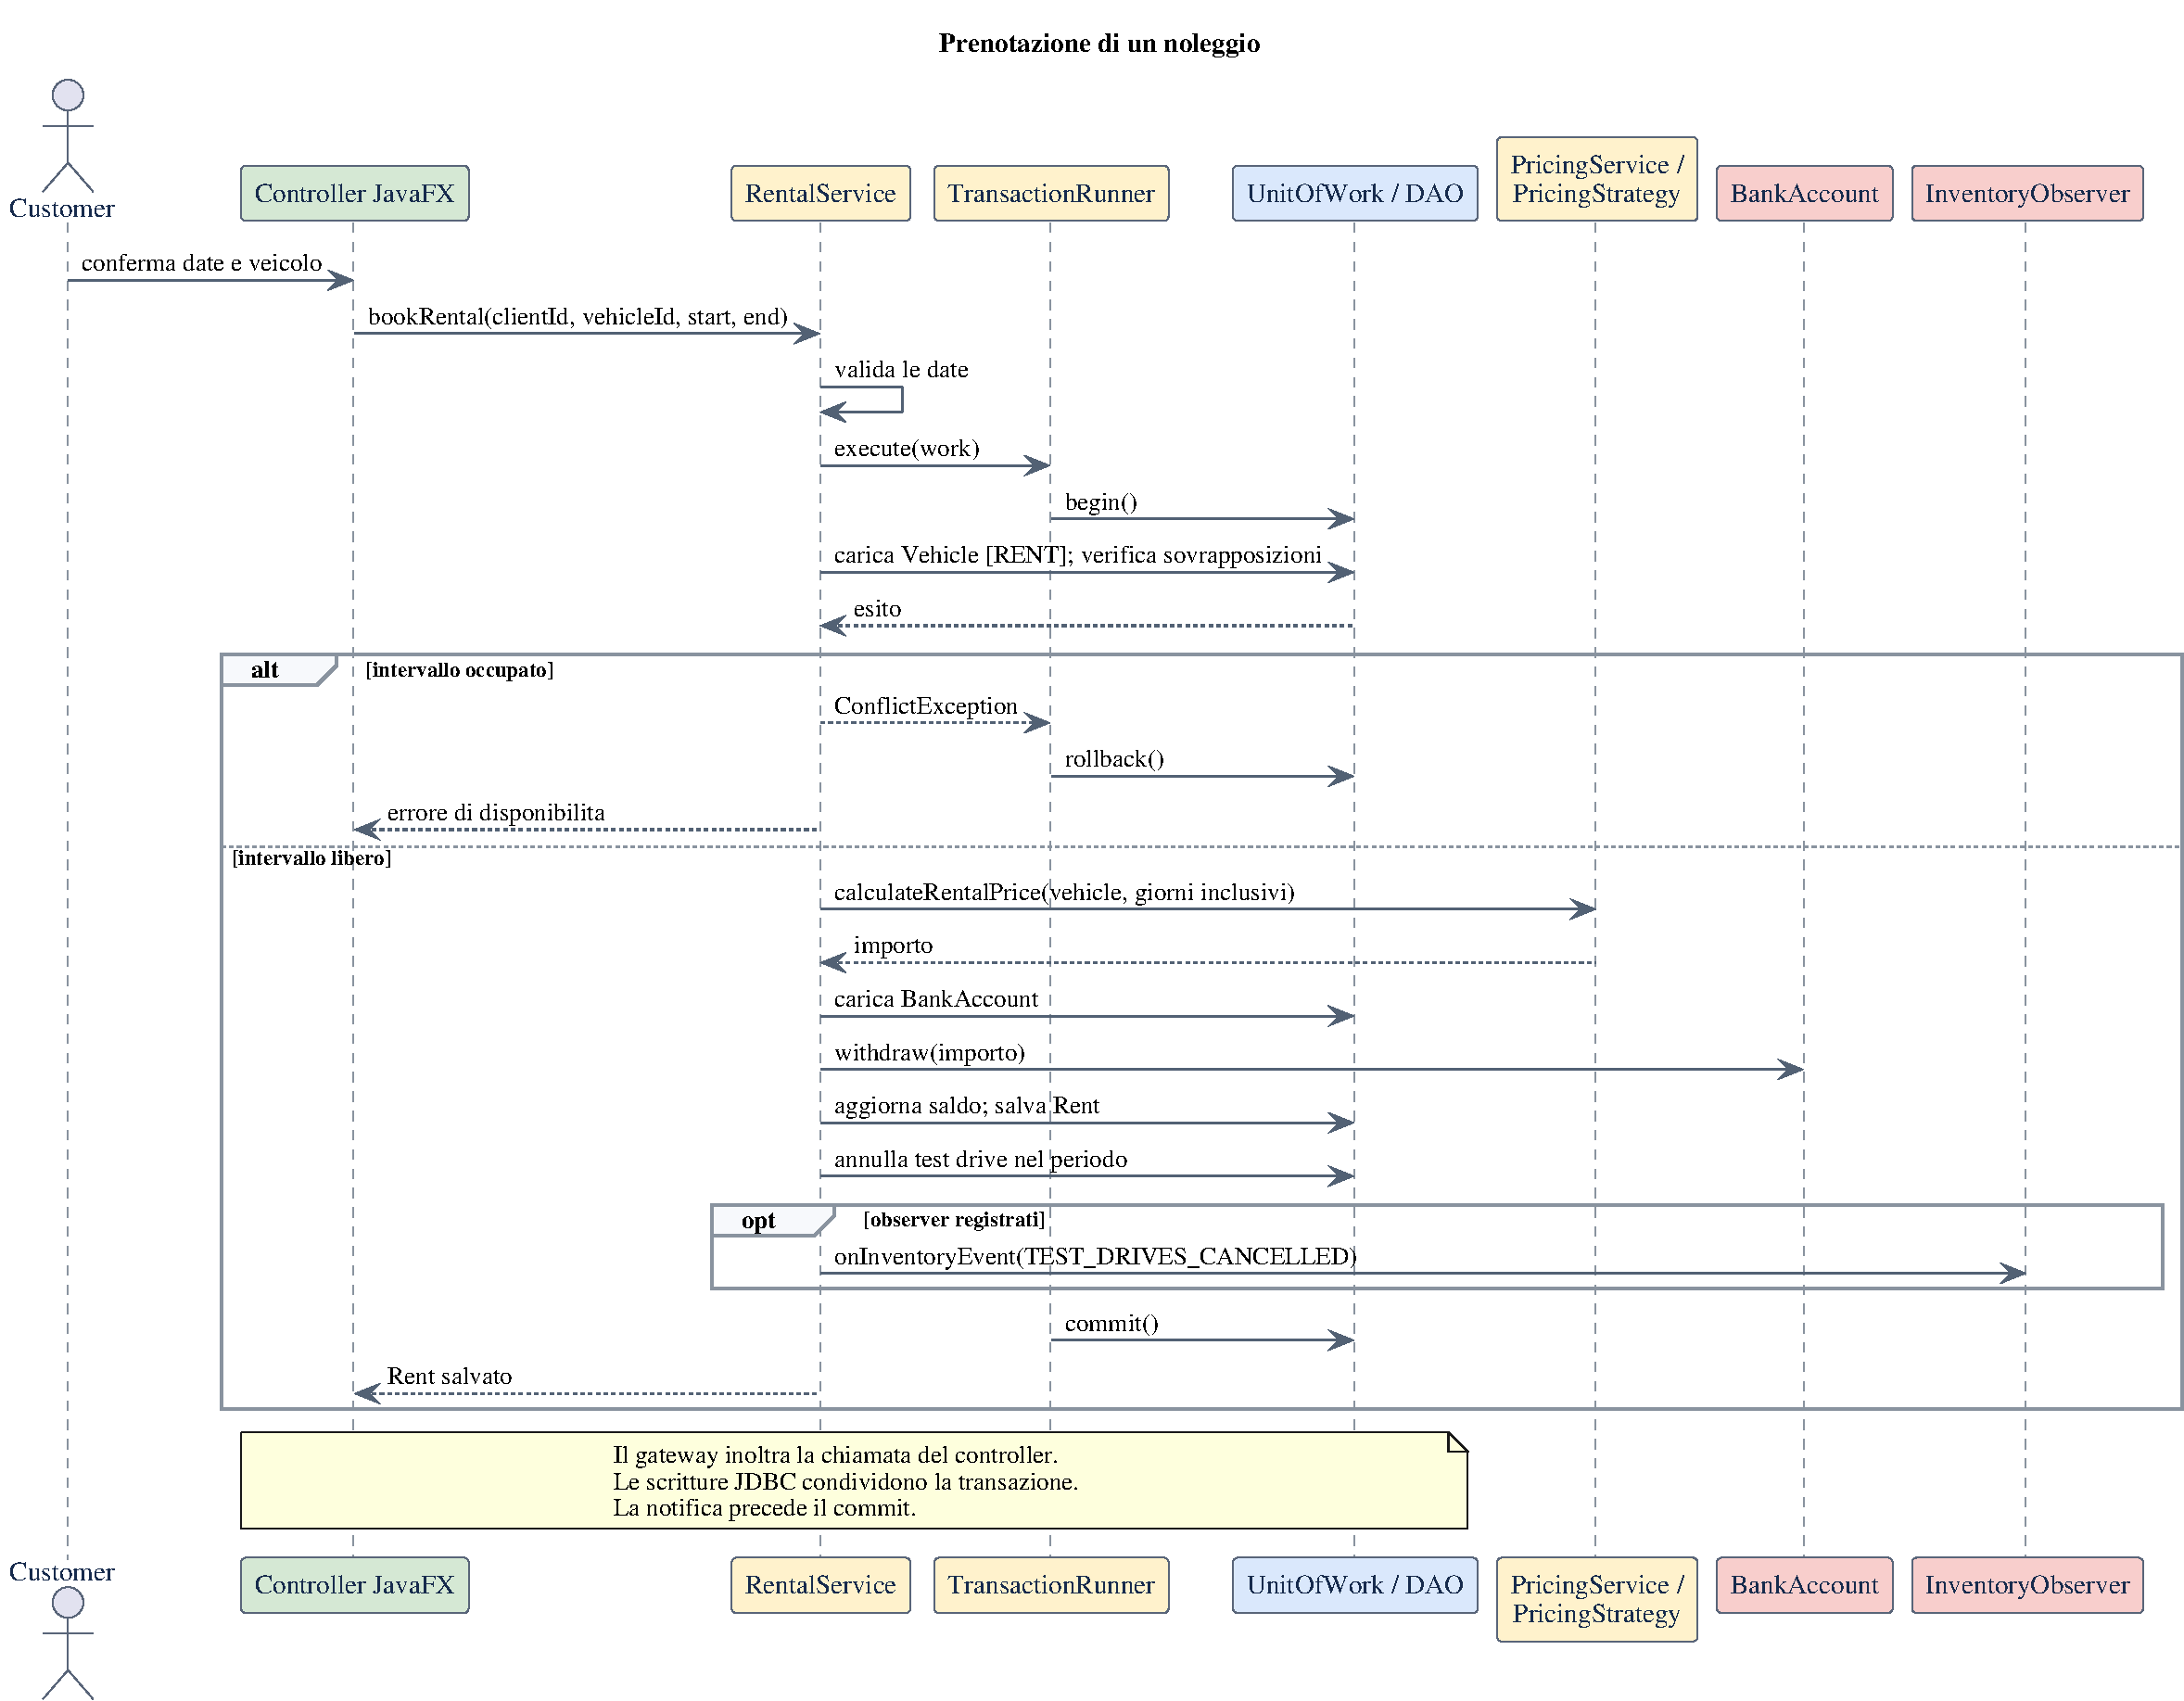
\includegraphics[width=\textwidth,height=.72\textheight,keepaspectratio]{sequence-rental-drivehub.pdf}
  \caption{Noleggio: controllo delle date, prezzo, addebito e registrazione nella stessa transazione.}\label{fig:seq-rental}
\end{figure}

La figura~\ref{fig:seq-rental} segue \code{RentalService.bookRental}. Il servizio valida le date, richiede che il veicolo sia in stato \code{RENT} e interroga il DAO per cercare noleggi sovrapposti. Se trova un conflitto, \code{TransactionRunner} esegue il rollback e la prenotazione non viene salvata. Nel percorso valido \code{PricingService} usa la \code{PricingStrategy} per calcolare l'importo sui giorni inclusivi; quindi il servizio addebita il conto dimostrativo, salva \code{Rent} e cancella i test drive nel periodo. La notifica a eventuali \code{InventoryObserver} precede il commit e non ha la stessa atomicità delle scritture JDBC. Il controllo di sovrapposizione è applicativo: nello schema non è presente un vincolo che escluda due prenotazioni concorrenti sullo stesso intervallo.

\clearpage
\subsection{Acquisizione di un veicolo del Customer}

\begin{figure}[H]
  \centering
  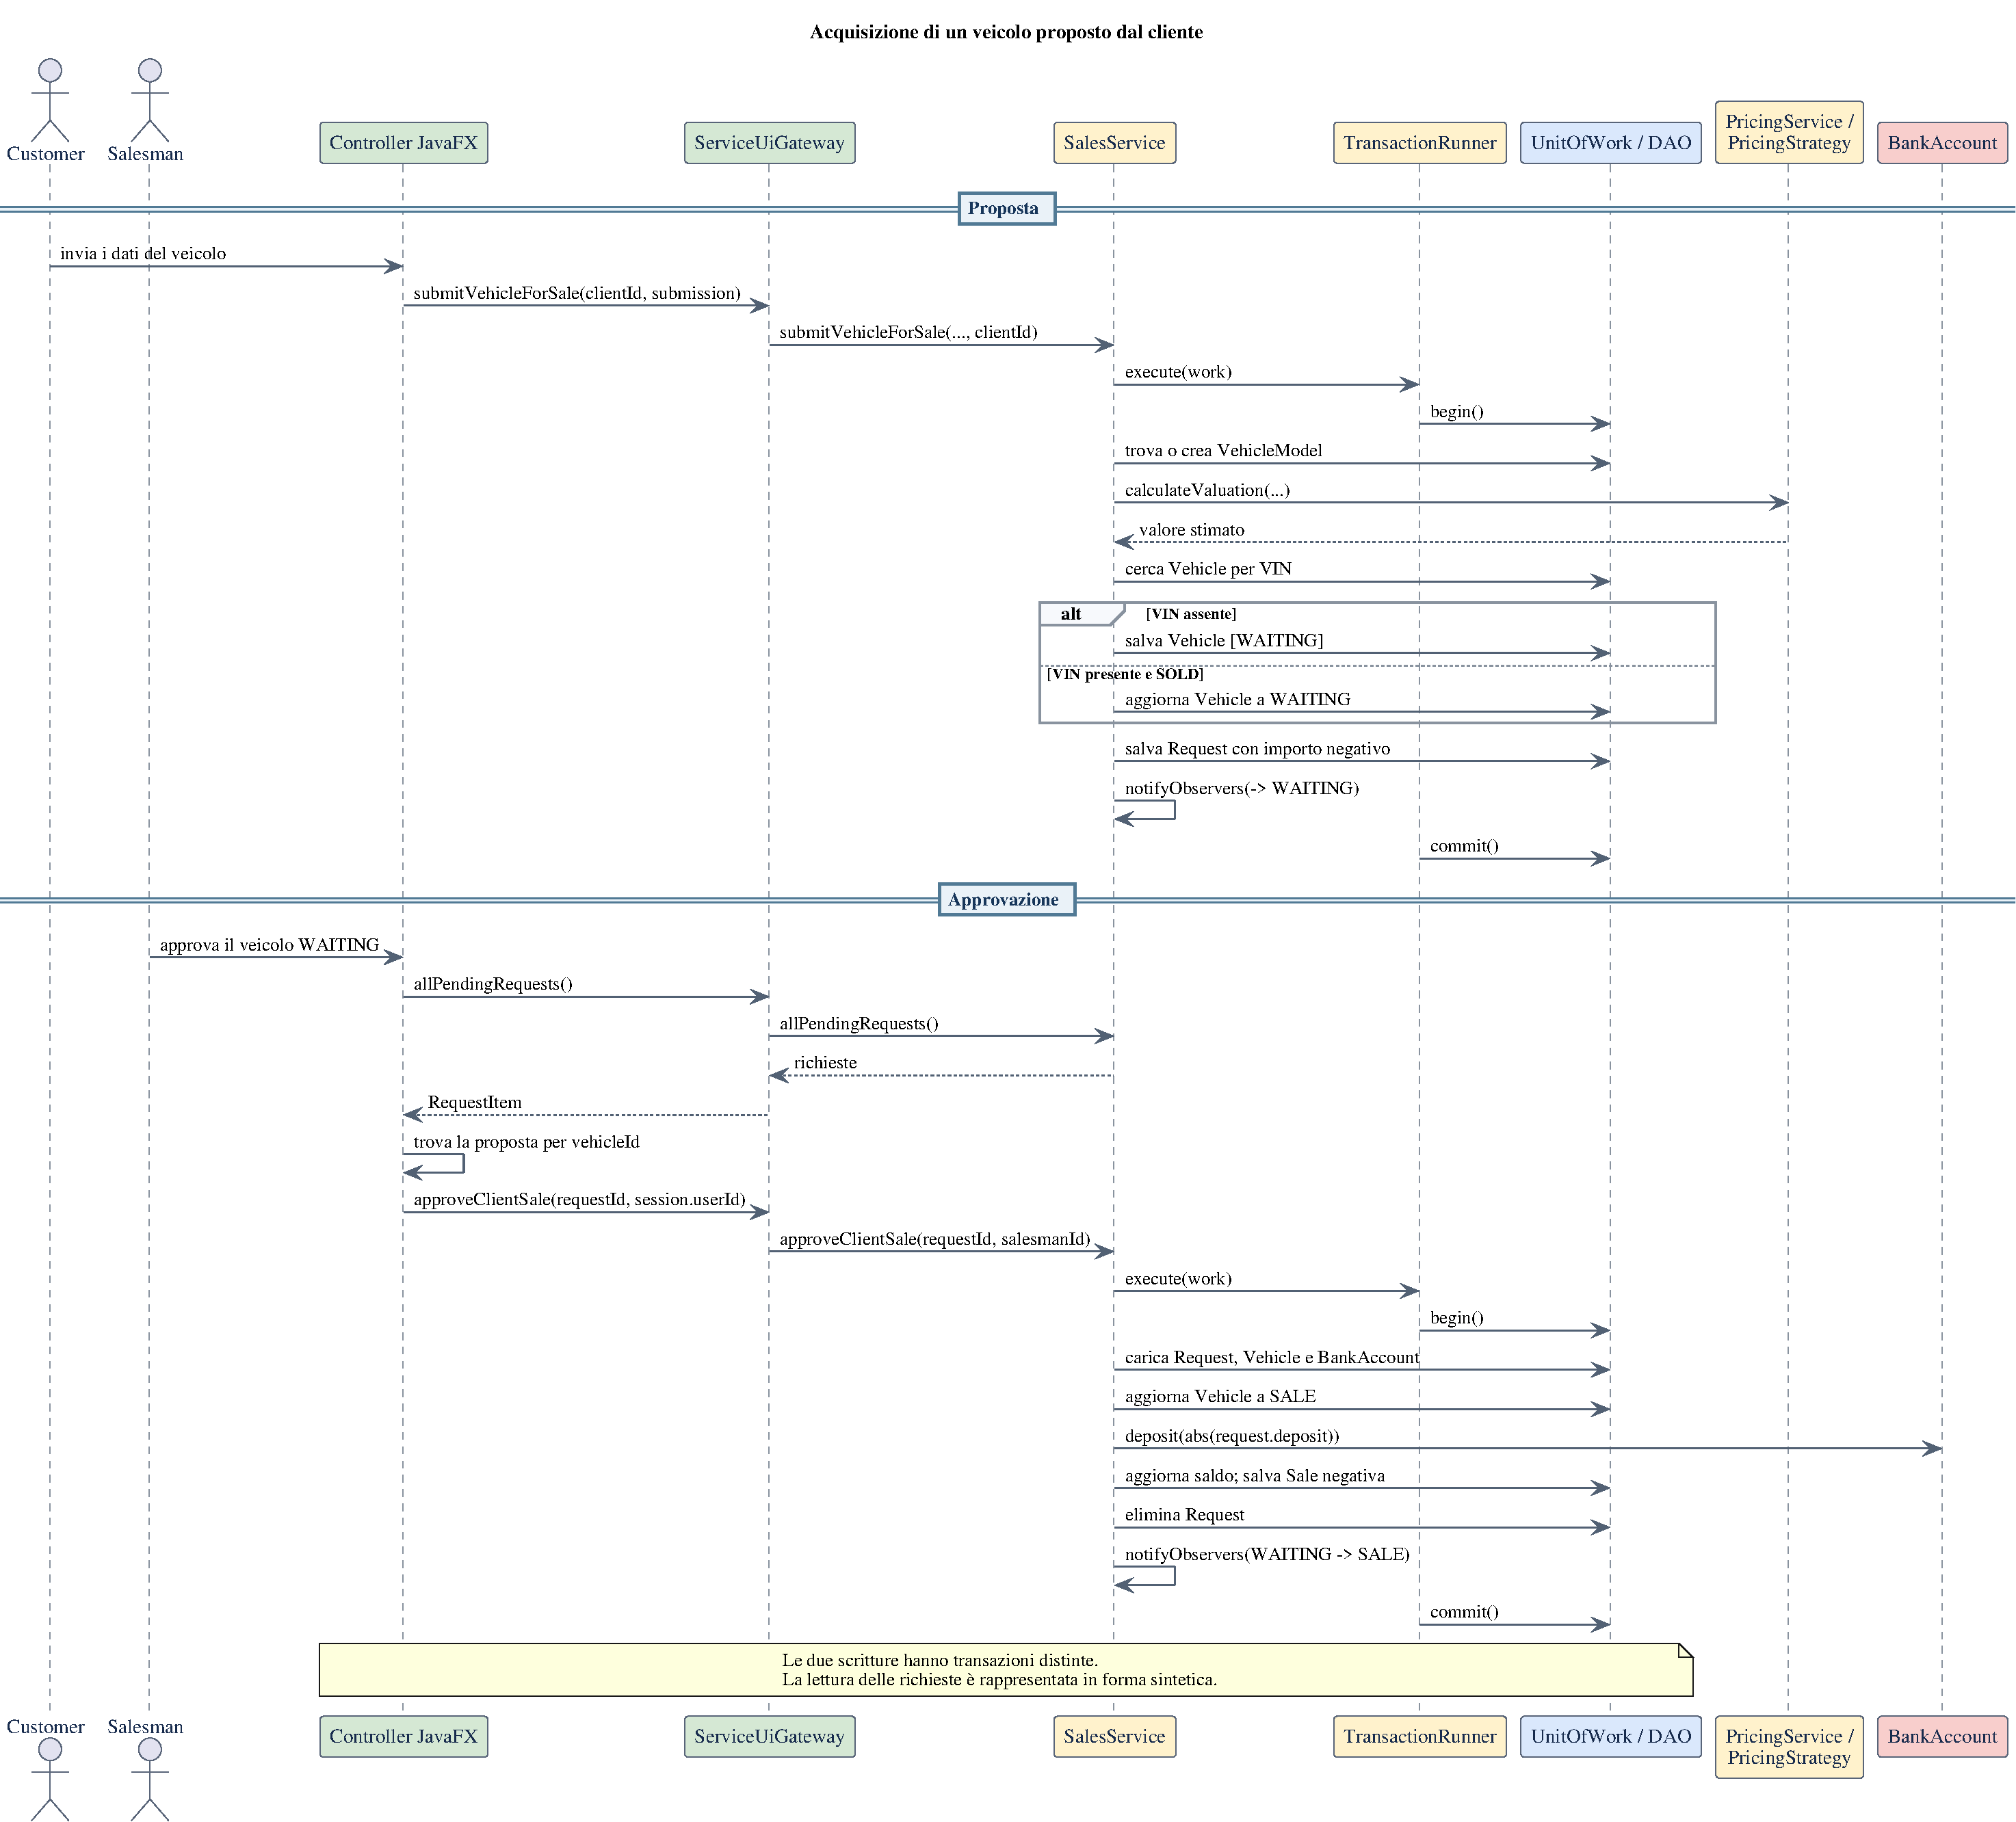
\includegraphics[width=\textwidth,height=.72\textheight,keepaspectratio]{sequence-acquisition-drivehub.pdf}
  \caption{Acquisizione: proposta del Customer e approvazione del Salesman, ciascuna in una transazione di scrittura.}\label{fig:seq-acquisition}
\end{figure}

Nella figura~\ref{fig:seq-acquisition}, la proposta crea o riusa un veicolo \code{SOLD}, lo pone in \code{WAITING} e salva una \code{Request} negativa. Il controller del Salesman cerca la richiesta di proposta per il veicolo selezionato e passa a \code{approveClientSale} l'ID del venditore in sessione. L'approvazione accredita il cliente, registra una \code{Sale} negativa, elimina la richiesta e porta il veicolo a \code{SALE} in una transazione. Il metodo \code{approveVehicle} è usato dal controller solo quando non trova una proposta; se chiamato direttamente su una proposta, apre invece due unità di lavoro annidate e usa l'ID venditore costante \code{1L}. La decisione appartiene al Salesman, non al Manager della specifica storica.
